\documentclass[../main.tex]{subfiles}

\begin{document}
\section{Preliminaries}\label{sec:preliminaries}
In this section we will review some basic concepts of linear algebra and vector calculus that will be used throughout the document.
\subsection{Properties of cross and dot products}
\begin{proposition}
  \label{prop:triplecross}
  Let $\vf{u}, \vf{v}, \vf{w}\in\RR^3$. Then:
  \begin{align}
    (\vf{u}\times\vf{v})\times\vf{w} & =(\vf{u}\cdot\vf{w})\vf{v}-(\vf{v}\cdot\vf{w})\vf{u} \\
    \vf{u}\times(\vf{v}\times\vf{w}) & =(\vf{u}\cdot\vf{w})\vf{v}-(\vf{u}\cdot\vf{v})\vf{w}
  \end{align}
\end{proposition}
\begin{proof}
  Let $\vf{u}=(u_1,u_2,u_3)$, $\vf{v}=(v_1,v_2,v_3)$, and $\vf{w}=(w_1,w_2,w_3)$. Then:
  \begin{align*}
    {((\vf{u}\times\vf{v})\times\vf{w})}_1 & =(u_3v_1-u_1v_3)w_3-(u_1v_2-u_2v_1)w_2                     \\
                                           & =(u_2w_2+u_3w_3)v_1-(v_2w_2+v_3w_3)u_1                     \\
                                           & =(u_1w_1+u_2w_2+u_3w_3)v_1-(v_1w_1+v_2w_2+v_3w_3)u_1       \\
                                           & ={((\vf{u}\cdot\vf{w})\vf{v}-(\vf{v}\cdot\vf{w})\vf{u})}_1
  \end{align*}
  The other components are treated similarly. The second equality follows in a similar way.
\end{proof}
\begin{proposition}
  Let $\vf{u}, \vf{v}, \vf{w}\in\RR^3$. Then:
  \begin{enumerate}
    \item $(\vf{u}\times\vf{v})\cdot\vf{w}=(\vf{u}\cdot\vf{w})\vf{v}\cdot\vf{w}-(\vf{v}\cdot\vf{w})\vf{u}\cdot\vf{w}$
  \end{enumerate}
\end{proposition}
\subsection{Conics in a nutshell}
\subsubsection{General conics}
\begin{definition}
  A conic is the curve obtained as the intersection of a plane with the surface of a double cone (a cone with two \emph{nappes}).
\end{definition}
In \cref{fig:conics}, we show the 3 types of conics: the ellipse, the parabola, and the hyperbola, which differ on their eccentricity, as we will see later on. Note that the circle is a special case of the ellipse.
\begin{figure}[htbp]
  \centering
  \begin{minipage}[t]{0.45\textwidth}
    \centering
    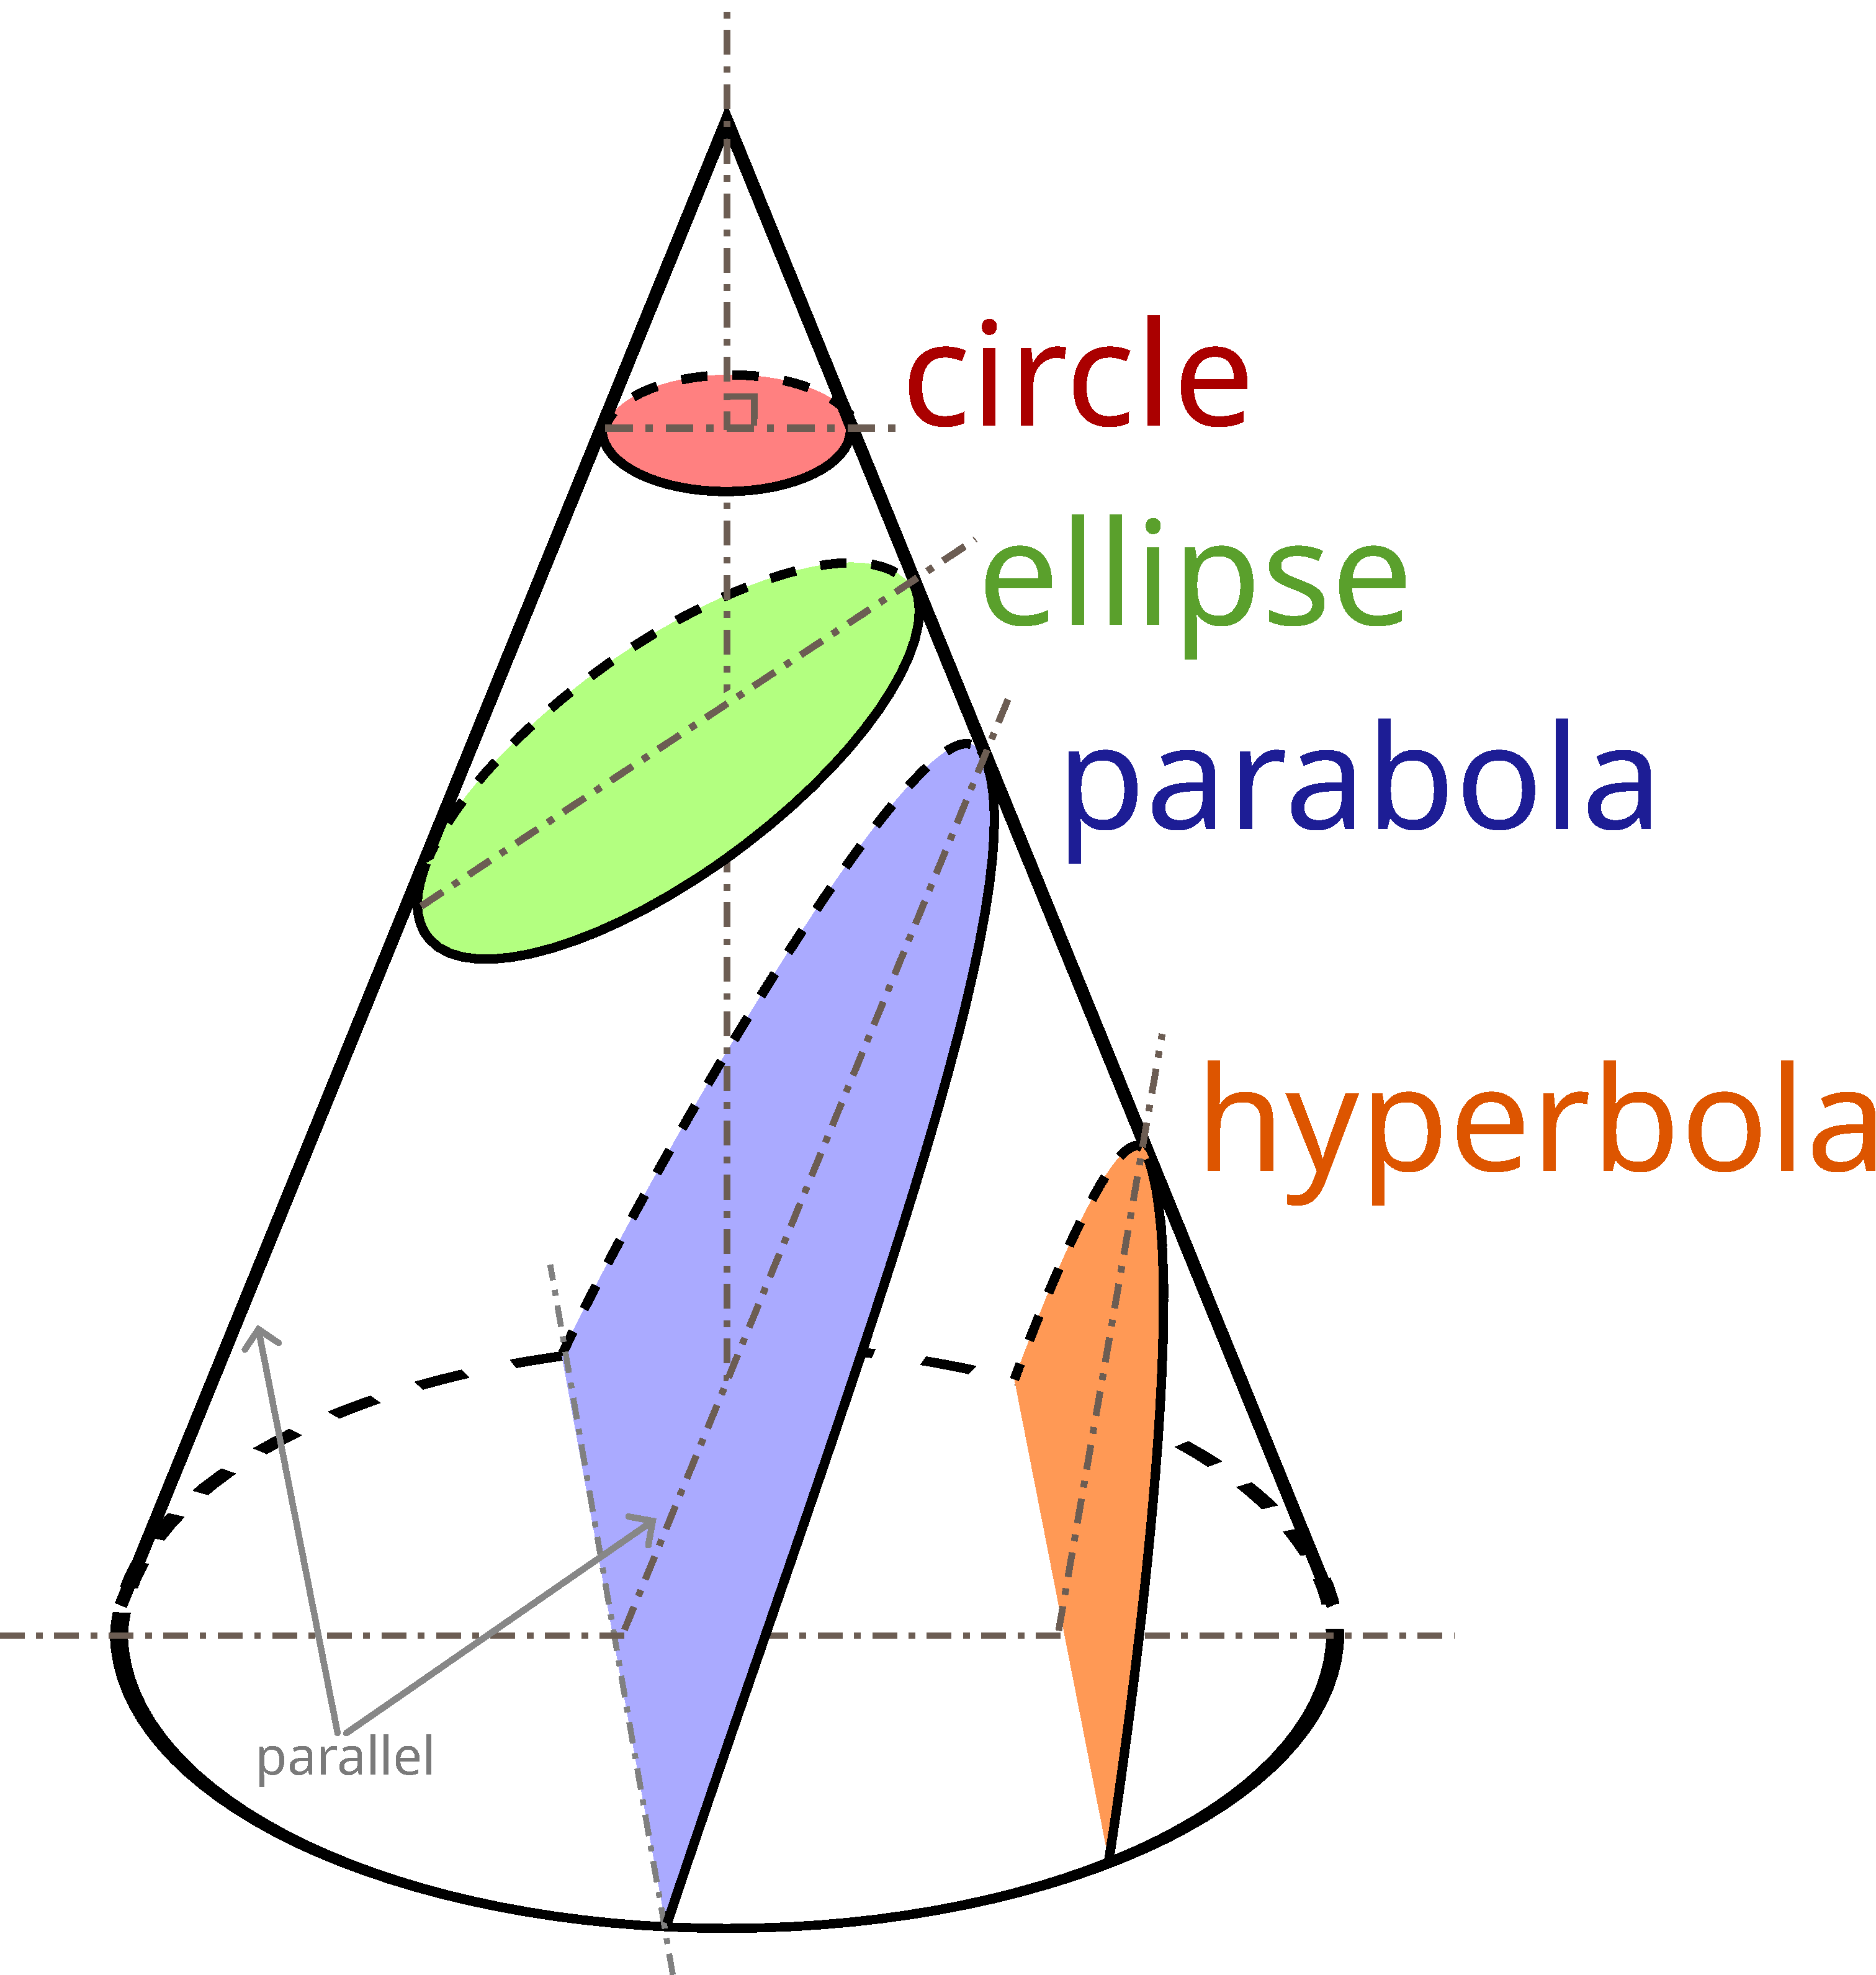
\includegraphics[width=\textwidth]{Images/Conic_Sections.pdf}
    \caption{The black boundaries of the colored regions are conic sections. The other half of the hyperbola, which is not shown, is in the other nappe of the double cone. (based on \cite{wiki:conic})}
    \label{fig:conics}
  \end{minipage}
  \hfill
  \begin{minipage}[t]{0.45\textwidth}
    \centering
    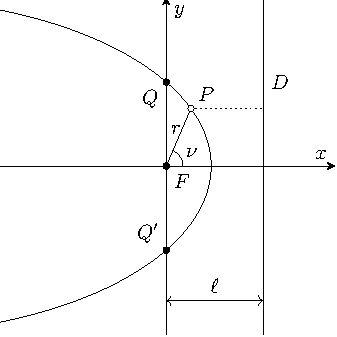
\includegraphics[width=\textwidth]{Images/conics.pdf}
    \caption{Reference frame centered at the focus of the conic and whose axes are such that the $y$-axis is parallel to the directrix and the $x$-axis is perpendicular to the directrix. The directions of the axes are chosen arbitrarily, subject to the constraint that a right-handed system $(x,y)$ is obtained.}
    \label{fig:conics_cartesian}
  \end{minipage}
\end{figure}

The following proposition gives a characterization of the conics.
\begin{proposition}
  A conic is the set of all points $P$ such that the distance from $P$ to a fixed point $F$ is a multiple of the distance from $P$ to a fixed line $D$. Mathematically, this is expressed as:
  \begin{equation}\label{eq:conic_pre}
    d(P,F)=e d(P,D)
  \end{equation}
  where $d$ is the Euclidean distance. The point $F$ is called the \emph{focus}; the line $D$, \emph{directrix}, and the constant of proportionality $e$, \emph{eccentricity}.
\end{proposition}
Note that using the polar coordinates $(r,\nu)$ centered at $F$ (as in \cref{fig:conics_cartesian}), we can rewrite \cref{eq:conic_pre} as:
\begin{equation}\label{eq:conic}
  r=e(\ell - r\cos\nu)\implies r= \frac{e\ell}{1+e\cos\nu}=:\frac{p}{1+e\cos\nu}
\end{equation}
where we have defined $p:=e\ell$.
\begin{definition}
  Le $C$ be a conic and $e$ be its eccentricity. We say that $C$ is
  \begin{itemize}
    \item an \emph{ellipse} if $0\leq e<1$,
    \item a \emph{parabola} if $e=1$, and
    \item a \emph{hyperbola} if $e>1$.
  \end{itemize}
  If $e=0$, the conic is called \emph{circle}.
\end{definition}
\subsubsection{Ellipse}\label{sec:ellipse}
From now on we will focus on the study of the ellipse. From \cref{eq:conic}, since $e<1$, it follows $r(\nu)$ is continuous. Therefore, the ellipse is bounded and closed conic section (and it is the only conic section satisfying these two properties).

Let's now study the extrema of $r(\nu)$. An easy check shows that the minimum is attained at $\nu=0$ and the maximum at $\nu=\pi$ and these values are given by:
\begin{equation}
  r_\mathrm{min}=\frac{p}{1+e}\qquad\text{and}\qquad r_\mathrm{max}=\frac{p}{1-e}
\end{equation}
When considering orbits of bodies these points are called \emph{periapsis} and \emph{apoapsis}, respectively\footnote{Other names are used in the literature when the the central body and the orbiter are particular ones. For example for the system Sun-Earth, the words \emph{perihelion} and \emph{aphelion} are used, whereas for the system Earth-Moon, the words \emph{perigee} and \emph{apogee} are used instead.}. The line connecting both points is called \emph{line of apsides}. Let's seek now the extrema of $x = r\cos\nu$ and $y = r\sin\nu$. Differentiating with respect to $\nu$ yields:
\begin{equation}
  x'=-\frac{p\sin\nu}{{(1+e\cos\nu)}^2}\qquad y'=\frac{p(e+\cos\nu)}{{(1+e\cos\nu)}^2}
\end{equation}
On the one hand, first expression vanishes at $\nu=0,\pi$. Therefore, the extrema of $x$ coincide with the periapsis and apoapsis points and at these points the $y$ coordinate is equal to 0. This means that the line of apsides passes through the focus of the ellipse. On the other hand, $y'$ vanishes at $\cos\nu=-e$. That is, at $\nu=\arccos (-e)$ and $\nu=2\pi-\arccos(-e)$. Therefore, using that $\sin(\arccos x)=\sqrt{1-x^2}$, the values of $y$ at these extrema are:
\begin{equation}
  y_\mathrm{min}=\frac{p}{1-e^2}\sin(\arccos(-e))=\frac{p}{\sqrt{1-e^2}}\qquad y_\mathrm{max}=\frac{p}{1-e^2}\sin(2\pi-\arccos(-e))=-\frac{p}{\sqrt{1-e^2}}
\end{equation}
Note that the $x$ coordinate at these two points is the same: $-\frac{pe}{1-e^2}$.
\begin{definition}
  Consider the reference frame \cref{fig:ellipse} centered at one focus. We define the \emph{semi-major axis} $a$ as half the segment that connects the two extrema of the $x$ coordinate. The \emph{semi-minor axis} $b$ is defined as half the segment that conects the two extrema of the $y$ coordinate. The length of those segments are also denoted by $a$ and $b$, respectively. Thus, these are given by the following expressions:
  \begin{equation}
    a:=\frac{r_\mathrm{max}+r_\mathrm{min}}{2}=\frac{p}{1-e^2}\qquad b:=\frac{y_\mathrm{max}+y_\mathrm{min}}{2}=\frac{p}{\sqrt{1-e^2}}
  \end{equation}
\end{definition}
From here note that we can express $b$ in terms of $a$ and $e$ as:
\begin{equation}\label{eq:ellipse_b_a}
  b=a\sqrt{1-e^2}
\end{equation}
\begin{definition}
  We define the center $O$ of the ellipse as the intersection of the semi-major axis and semi-minor axis.
\end{definition}
Let's calculate the distance from the focus $F$ to one of the extrema of the $y$ coordinate.
\begin{equation}
  d\left(F,\left(-\frac{pe}{1-e^2},\pm \frac{p}{\sqrt{1-e^2}}\right)\right)=\frac{p}{\sqrt{1-e^2}}\sqrt{\frac{e^2}{1-e^2}+1}=\frac{p}{1-e^2}=a
\end{equation}
Hence, the value of $c$ in \cref{fig:ellipse} can be simplified to:
\begin{equation}
  c^2=a^2-b^2=a^2-a^2(1-e^2)=a^2e^2\implies c=ae
\end{equation}
\begin{figure}
  \centering
  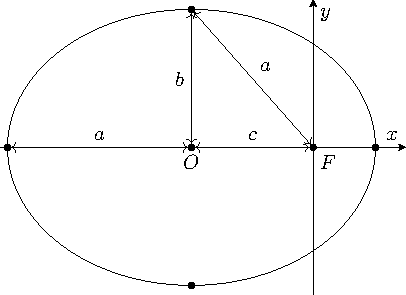
\includegraphics[width=0.5\textwidth]{Images/ellipse.pdf}
  \caption{Ellipse}
  \label{fig:ellipse}
\end{figure}
\begin{proposition}
  The area enclosed in a ellipse of semi-major axis $a$ and semi-minor axis $b$ is $\pi a b$.
\end{proposition}
\begin{proof}
  Consider the ellipse $E$ centered at the origin and oriented as in \cref{fig:ellipse}. From \cref{fig:ellipse} one can see that it can be parametrized by $(x,y)=(\frac{p\cos\nu}{1-e^2}+ae,\frac{p\sin\nu}{1+e\cos\nu})$ with $\nu\in[0,2\pi)$. An easy check shows that this parametrization satisfies:
  \begin{equation}
    \frac{x^2}{a^2}+\frac{y^2}{b^2}=1
  \end{equation}
  Hence, the area enclosed in the ellipse is can be parametrized by $(x, y)=(ar\cos\nu,br\sin\nu)$, with $r\in[0,1]$ and $\nu\in[0,2\pi]$. The Jacobian of this transformation is $abr$. Therefore, from the change of variable theorem we have that:
  \begin{equation}
    \mathrm{Area}(E)=\iint_E\dd{x}\dd{y}=\int_{0}^{2\pi}\int_{0}^{1}rab\dd{r}\dd\nu=\pi ab
  \end{equation}
\end{proof}
\subsection{Spherical harmonics}
\subsubsection{Legendre polynomials, regularity and orthonormality}
\begin{definition}
  Consider the following second-order differential equation called \emph{Legendre differential equation}:
  \begin{equation}
    (1-x^2)y''-2xy'+\lambda y=0
  \end{equation}
  for $\lambda\in\RR$. This equation can be rewritten as:
  \begin{equation}\label{eq:legendre_diff_eq}
    {((1-x^2)y')}'+\lambda  y=0
  \end{equation}
\end{definition}
If seek for analytic solutions of this equation using the power series method \cite{florida:legendre}, i.e. looking for solutions of the form $y(x)=\sum_{j=0}^{\infty}a_jx^j$, we see that:
\begin{multline}
  0=(1-x^2)\sum_{j=0}^{\infty}a_{j+2}(j+1)(j+2)x^j-2x\sum_{j=0}^{\infty}a_{j+1}(j+1)x^j+\lambda\sum_{j=0}^{\infty}a_jx^j =\sum_{j=0}^{\infty}a_{j+2}(j+1)(j+2)x^j-\\-\sum_{j=0}^{\infty}a_{j}(j-1)jx^{j}-\sum_{j=0}^{\infty}2a_{j}jx^{j}+\sum_{j=0}^{\infty}\lambda a_jx^j  =\sum_{j=0}^{\infty}[a_{j+2}(j+1)(j+2) - a_j(j(j+1)-\lambda)]x^j
\end{multline}
Equating the general term of the series equal to 0 we obtain this recursion:
\begin{equation}\label{eq:legendre_recursion}
  a_{j+2}=\frac{j(j+1)-\lambda}{(j+1)(j+2)}a_j\quad j=0,1,2,\ldots
\end{equation}
From here we can obtain two independent solutions by setting the initial conditions $a_0$ and $a_1$ of the iteration. For example, setting $a_1=0$ we obtain a series that has only even powers of $x$. On the other hand, setting $a_0=0$ we obtain a series that has only odd powers of $x$. These two series converge on the interval $(-1,1)$ by the ratio test (by looking at \cref{eq:legendre_recursion}) and can be expressed compactly as \cite{florida:legendre}:
\begin{equation}\label{eq:legendre_series}
  y_\mathrm{e}(x)=a_0\sum_{j=0}^{\infty}\left[\prod_{k=0}^{j-1}(2k(2k+1)-\lambda)\right]\frac{x^{2j}}{(2j)!}\quad y_\mathrm{o}(x)=a_1\sum_{j=0}^{\infty}\left[\prod_{k=0}^{j-1}((2k+1)(2k+2)-\lambda)\right]\frac{x^{2j+1}}{(2j+1)!}
\end{equation}
Here the empty product (that is, for instance when $k$ ranges from 0 to $-1$) is defined to be 1. However for each $\lambda\in\RR$ either one of these series or both diverge at $x=\pm 1$, as they behave as the harmonic series in a neighbourhood of $x=\pm 1$. We are interested, though, in the solutions that remain bounded on the whole interval $[-1,1]$. Looking at the expressions of \cref{eq:legendre_series} one can check that the only possibility to make the series converge in $[-1,1]$ is when $\lambda =n(n+1)$, $n\in\NN\cup\{0\}$. In this case, for each $n\in\NN\cup\{0\}$ exactly one of the series is in fact a polynomial of degree $n$. If, furthermore, we choose $a_0$ or $a_1$ be such that the polynomial evaluates to 1 at $x=1$, these polynomials are called \emph{Legendre polynomials} and they are denoted by $P_n(x)$. The other (divergent) series is usually denoted in the literature by $Q_n(x)$ (check \cite{mathematical_methods,florida:legendre}). And so the general solution of \cref{eq:legendre_diff_eq} for $\lambda=n(n+1)$ can be expressed as a linear combination of $P_n$ and $Q_n$, because the space of solutions form a vector space of dimension 2.

\begin{figure}[ht]
  \centering
  \begin{minipage}[ht]{0.48\textwidth}
    \centering
    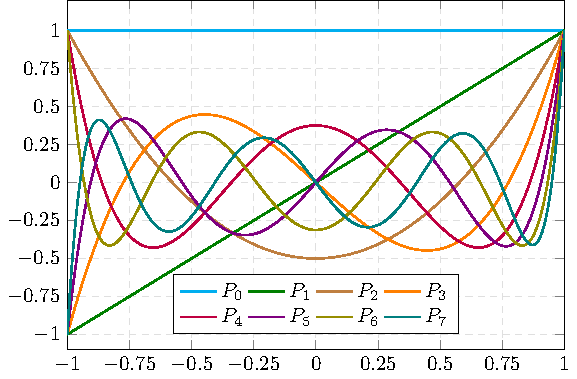
\includegraphics[width=\textwidth]{Images/legendre.pdf}
    \caption{Graphic representation of the first eight Legendre polynomials.}
  \end{minipage}
  \hfill
  \begin{minipage}[ht]{0.48\textwidth}
    \centering
    \captionsetup{type=table} %% tell latex to change to table
    \begin{tabular}{c|c}
      $n$ & $P_n(x)$                                 \\
      \hline\hline
      $0$ & $1$                                      \\
      $1$ & $x$                                      \\
      $2$ & $\frac{1}{2}(3x^2-1)$                    \\
      $3$ & $\frac{1}{2}(5x^3-3x)$                   \\
      $4$ & $\frac{1}{8}(35x^4-30x^2+3)$             \\
      $5$ & $\frac{1}{8}(63x^5-70x^3+15x)$           \\
      $6$ & $\frac{1}{16}(231x^6-315x^4+105x^2-5)$   \\
      $7$ & $\frac{1}{16}(429x^7-693x^5+315x^3-35x)$ \\
    \end{tabular}
    \caption{First eight Legendre polynomials}
    \label{tab:legendre_polys}
  \end{minipage}
\end{figure}
% The following proposition gives and explicit formula for the Legendre polynomials.
% \begin{proposition}[Rodrigues' formula]
%   Let $n\in \NN\cup\{0\}$. Then, $\forall x\in[-1,1]$:
%   \begin{equation}\label{eq:rodrigues}
%     P_n(x)=\frac{1}{2^n n!}\dv[n]{}{x}\left[{\left(x^2-1\right)}^n\right]
%   \end{equation}
% \end{proposition}
% \textcolor{red}{\begin{proposition}
%     Consider the function $g_x(t)=\frac{1}{\sqrt{1-2xt+t^2}}$ with $\abs{x}\leq 1$. Then, the generating function of $g$ is:
%     \begin{equation}
%       \frac{1}{\sqrt{1-2xt+t^2}}=\sum_{n=0}^{\infty}P_n(x)t^n
%     \end{equation}
%   \end{proposition}
%   \begin{proof}
%     Assume that formally $\frac{1}{\sqrt{1-2xt+t^2}}=\sum_{n=0}^{\infty}Q_n(x)t^n$. We want to check that $Q_n(x)=P_n(x)$ for all $n\in\NN\cup\{0\}$. Differentiating the equation with respect to $x$ and with respect to $t$ we obtain:
%     \begin{equation}\label{eq:rec_legendre_proof}
%       \frac{x-t}{{(1-2xt+t^2)}^{3/2}}=\sum_{n=0}^{\infty}nQ_n(x)t^{n-1}\qquad\frac{t}{{(1-2xt+t^2)}^{3/2}}=\sum_{n=0}^{\infty}{Q_n}'t^n
%     \end{equation}
%     The second equation can be rewritten as:
%     \begin{equation}
%       t\sum_{n=0}^{\infty}Q_n t^n=(1-2xt+t^2)\sum_{n=0}^{\infty}{Q_n}'(x)t^{n-1}
%     \end{equation}
%     So equating the coefficients of $t^n$ we get:
%     \begin{equation}
%       Q_{n}={Q_{n+1}}'-2x{Q_n}'+{Q_{n-1}}'
%     \end{equation}
%     Moreover, from \cref{eq:rec_legendre_proof} we have that:
%     \begin{equation}
%       t\sum_{n=0}^{\infty}nQ_n(x)t^{n-1}=(x-t)\sum_{n=0}^{\infty}{Q_n}'(x)t^{n}
%     \end{equation}
%     Again equating the coefficients of $t^n$ we get:
%     \begin{equation}
%       nQ_n=x{Q_n}'-{Q_{n-1}}'
%     \end{equation}
%     Hence differentiating $(1-x^2){P_n}'$ we have:
%     \begin{equation}
%       {((1-x^2){P_n}')}'=-2x{P_n}'+(1-x^2)P
%     \end{equation}
%     \textcolor{red}{NOT FINISHED!!!!!!!!!!}
%   \end{proof}}
The following proposition will be of our interest in the next section \cite{mathematical_methods}.
\begin{proposition}\label{prop:associate_legendre}
  Let $y(x)$ be a solution to the Legendre differential equation. Then, $\forall m\in\NN\cup\{0\}$ the function
  \begin{equation}
    w_m(x)={(1-x^2)}^{m/2} \dv[m]{y(x)}{x}
  \end{equation}
  solves the \emph{general Legendre differential equation}:
  \begin{equation}
    (1-x^2)y''-2xy'+\left(\lambda - \frac{m^2}{1-x^2}\right) y=0
  \end{equation}
  In particular if $\lambda=n(n+1)$ for $n\in\NN\cup\{0\}$, then $w_m(x)$ is denoted as
  \begin{equation}\label{eq:associated_legendre_polynomials}
    P_{n,m}(x):={(1-x^2)}^{m/2} \dv[m]{P_n}{x}
  \end{equation}
  and it is called the \emph{associated Legendre polynomial} of degree $n$ and order $m$.
\end{proposition}
% \begin{proof}
%   We know that $P_n$ satisfies the equation:
%   \begin{equation}\label{eq:proof_aso1}
%     (1-x^2)P_n''-2xP_n'+n(n+1)P_n=0
%   \end{equation}
%   Recall the Leibniz rule for differentiation:
%   \begin{equation}
%     {(fg)}^{(m)}=\sum_{k=0}^{m}\binom{m}{k}f^{(m-k)}g^{(k)}
%   \end{equation}
%   Differentiating \cref{eq:proof_aso1} $m$ times using the Leibniz rule and letting $v=\dv[m]{P_n}{x}$ we obtain:
%   \begin{equation}
%     [(1-x^2)v''-2xm v'-m(m-1)v]-[2xv'+2mv]+n(n+1)v= (1-x^2)v''-2x(m+1)v'+(n-m)(n+m+1)v=0
%   \end{equation}
%   Now let $P_{n,m}(x)={(1-x^2)}^{m/2}v$. Using the chain rule and isolating $v'$ and $v''$ we obtain:
%   \begin{align*}
%     {P_{n,m}}'= {(1-x^2)}^{m/2}v' - \frac{m}{2}x{(1-x^2)}^{m/2-1}v={(1-x^2)}^{m/2}v' - \frac{m}{2}\frac{P_{n,m}}{1-x^2}\implies v'= \frac{2}{m}\frac{1-x^2}{x}P_{n,m} - \frac{2}{m}x{P_{n,m}}' \\
%   \end{align*}
%   ....
% \end{proof}
Note that although these functions $P_{n,m}$ are named as \emph{polynomials}, they are only \emph{true} polynomials when $m$ is even. But we have opt to call them in that manner as it is the common practice in the literature (see \cite{wolfram_associated_legendre_polynomials,mathematical_methods,florida:legendre}).

Moreover, from the definition of $P_{n,m}$, we can see $P_{n,0}=P_n$ and that $P_{n,m}=0$ if $m>n$. So we can restrict the domain of $m$ to the set $\{0,1,\dots,n\}$.

% Finally, putting \cref{eq:associated_legendre_polynomials,eq:rodrigues} together, we obtain the following explicit formula for the associated Legendre polynomials:
% \begin{equation}
%   P_{n,m}(x)=\frac{1}{2^n n!}{(1-x^2)}^{m/2} \dv[n+m]{x}\left[{\left(x^2-1\right)}^n\right]
% \end{equation}
% This allows us to extend the range of $m$ to $\{-n,-(n-1),\dots,n-1,n\}$.
% \begin{lemma}\label{lem:neg_asso_legendre}
%   Let $n\in\NN\cup\{0\}$ and $m\in\{0,\ldots,n\}$. Then:
%   \begin{equation}
%     P_n^{-m}(x)=(-1)^m \frac{(n-m)!}{(n+m)!}P_{n,m}(x)
%   \end{equation}
% \end{lemma}
% This lemma shows us that the new extended associated polynomials $P_n^{-m}$, $m\in\{0,\ldots,n\}$, are also solutions to the general Legendre differential equation because the satisfy the same equation as $P_{n,m}$ and they only differ by a constant factor.
% My spherical harmonics are the same as the ones in Riley, Hobson, Bence except for the minus sign (-1)^m in front of Y_{n,m}^{\mathrm{c}}.  
\begin{table}[ht]
  \centering
  \captionsetup{type=table} %% tell latex to change to table
  \begin{tabular}{c|c||c|c}
    $n$ & $P_{n,1}(x)$                              & $n$ & $P_{n,2}(x)$                          \\
    \hline
    $1$ & $\sqrt{1-x^2}$                            & $2$ & $3(1-x^2)$                            \\
    $2$ & $3x\sqrt{1-x^2}$                          & $3$ & $15x(1-x^2)$                          \\
    $3$ & $\frac{3}{2}(5 x^2-1)\sqrt{1-x^2}$        & $4$ & $\frac{15}{2}(7x^2-1)(1-x^2)$         \\
    $4$ & $\frac{5}{2}x(7x^2-3)\sqrt{1-x^2}$        & $5$ & $\frac{105}{2}x(3x^2-1)(1-x^2)$       \\
    $5$ & $\frac{15}{8}(21x^4-14x^2+1)\sqrt{1-x^2}$ & $6$ & $\frac{105}{8}(33x^4-18x^2+1)(1-x^2)$ \\
  \end{tabular}
  \caption{First associated Legendre polynomials for $m=1$ and $m=2$.}
\end{table}
\begin{figure}[ht]
  \centering
  \begin{subfigure}[b]{0.48\textwidth}
    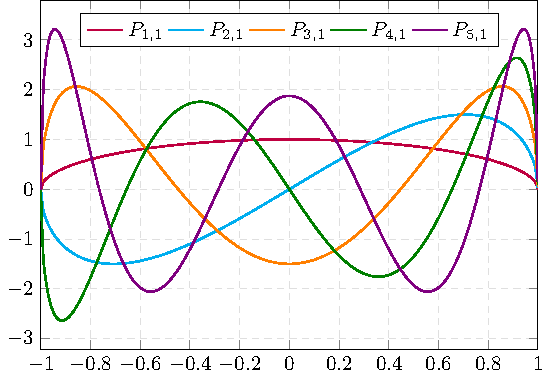
\includegraphics[width=\textwidth]{Images/assolegendre1.pdf}
    \caption{$m=1$}
  \end{subfigure}
  \quad
  \begin{subfigure}[b]{0.48\textwidth}
    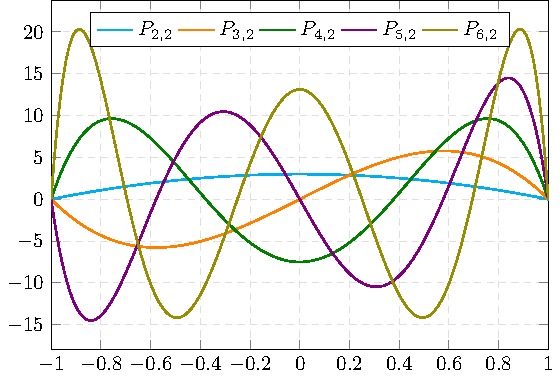
\includegraphics[width=\textwidth]{Images/assolegendre2.pdf}
    \caption{$m=2$}
  \end{subfigure}
  \caption{Graphic representation of the first associated Legendre polynomials for $m=1$ and $m=2$.}
\end{figure}
\begin{definition}
  Let $n\in\NN\cup\{0\}$ and $m\in\{0,1,\dots,n\}$. We define the \emph{real spherical harmonics} $Y_{n,m}^{\mathrm{c}}$ and $Y_{n,m}^{\mathrm{s}}$ as:
  \begin{align}
    Y_{n,m}^{\mathrm{c}}(\theta,\phi) & =\sqrt{(2-\delta_{0,m})(2n+1)\frac{(n-m)!}{(n+m)!} }P_{n,m}(\cos\phi) \cos{m\theta} \\
    Y_{n,m}^{\mathrm{s}}(\theta,\phi) & =\sqrt{(2-\delta_{0,m})(2n+1)\frac{(n-m)!}{(n+m)!} }P_{n,m}(\cos\phi) \sin{m\theta}
  \end{align}
  The factor $N_{n,m}:=\sqrt{(2-\delta_{0,m})(2n+1)\frac{(n-m)!}{(n+m)!} }$ is called the \emph{normalization factor} of the spherical harmonics and $\delta_{0,m}$ is the Kronecker delta. The weird factor $2-\delta_{0,m}$ in $N_{n,m}$ will become clear in the next section.
\end{definition}
\begin{table}[ht]
  \centering
  \captionsetup{type=table} %% tell latex to change to table
  \begin{tabular}{c|c|c||c|c|c}
    $n$ & $m$ & $Y_{n,1}^{\mathrm{c}}(\theta,\phi)$     & $n$ & $m$ & $Y_{n,2}^{\mathrm{c}}(\theta,\phi)$                        \\
    \hline
    $0$ & 0   & $1$                                     & $2$ & 2   & $\frac{\sqrt{15}}{2}{(\sin\phi)}^2\cos 2\theta$            \\
    $1$ & 0   & $\sqrt{3}\cos\phi$                      & $3$ & 0   & $\frac{\sqrt{7}}{2}\cos\phi(5{(\cos\phi)}^2-3)$            \\
    $1$ & 1   & $\sqrt{3}\sin\phi\cos\theta$            & $3$ & 1   & $\frac{\sqrt{42}}{4}(5{(\cos\phi)}^2-1)\sin\phi\cos\theta$ \\
    $2$ & 0   & $\frac{\sqrt{5}}{2}(3{(\cos\phi)}^2-1)$ & $3$ & 2   & $\frac{\sqrt{105}}{2}{(\sin\phi)}^2\cos\phi\cos 2\theta$   \\
    $2$ & 1   & $\sqrt{15}\sin\phi\cos\phi\cos\theta$   & $3$ & 3   & $\frac{\sqrt{70}}{4}{(\sin\phi)}^3\cos 3\theta$            \\
  \end{tabular}
  \caption{First cosine spherical harmonics.}
\end{table}
\begin{figure}[ht]
  \centering
  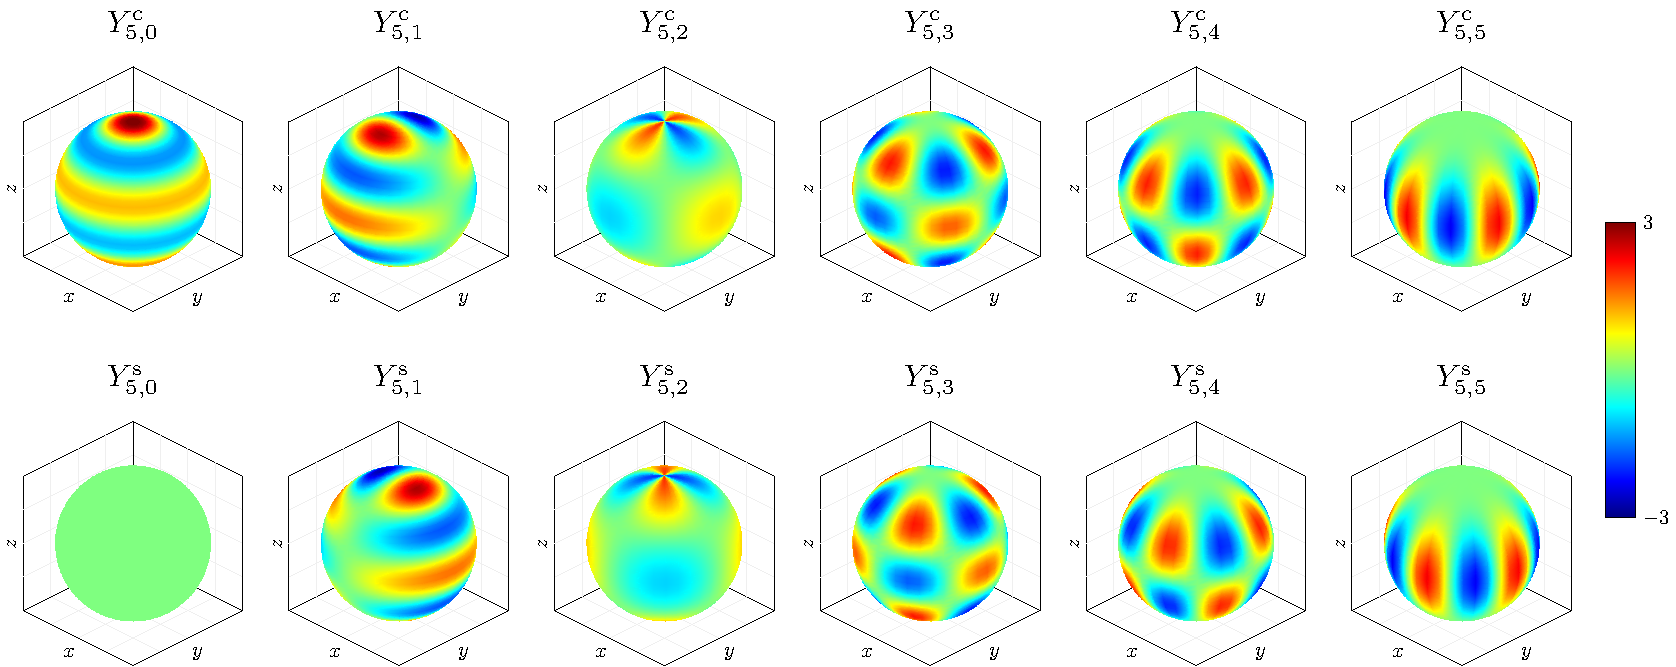
\includegraphics[width=\textwidth]{Images/sphericalHarmonics.pdf}
  \caption{3D heat map of the spherical harmonics of degree $n=5$. The first row correspond to the cosine spherical harmonics and the second row correspond to the sine spherical harmonics.}
\end{figure}

\subsubsection{Laplace equation in spherical coordinates}\label{sec:laplace_spherical}
\begin{definition}
  Let $f:\RR^3\rightarrow\RR$ be a twice-differentiable function. The \emph{Laplace equation} is the equation
  \begin{equation}
    \laplacian f=\pdv[2]{f}{x}+\pdv[2]{f}{y}+\pdv[2]{f}{z}=0
  \end{equation}
  where $\Delta$ is the Laplace operator.
\end{definition}
The next proposition gives the Laplace equation in spherical coordinates.
\begin{proposition}
  Let $f:\RR^3\rightarrow\RR$ be a twice-differentiable function. Then:
  \begin{equation}\label{eq:laplace}
    \frac{1}{r^2}\pdv{}{r}\left(r^2\pdv{f}{r}\right)+\frac{1}{r^2\sin\phi}\pdv{}{\phi}\left(\sin\phi\pdv{f}{\phi}\right)+\frac{1}{r^2{(\sin\phi)}^2}\pdv[2]{f}{\theta}=0
  \end{equation}
  where $r$ denotes the radial distance, $\theta$ denotes the azimuthal angle, and $\phi$, the polar angle (or colatitude).
\end{proposition}
We are now interested in solving the Laplace equation. \cref{thm:laplace_spherical} gives the solution of it as a function of the spherical harmonics.
\begin{theorem}\label{thm:laplace_spherical}
  The regular solutions in a bounded region $\Omega\subseteq \RR^3$ such that $0\notin\overline{\Omega}$ to the Laplace equation in spherical coordinates are of the form
  \begin{align}
    f(r,\theta,\phi) & = \sum_{n=0}^\infty \sum_{m=0}^n (a_n r^{n} +b_{n}r^{-n-1})P_{n,m}(\cos\phi) (c_{n,m}\cos(m\theta)+s_{n,m}\sin(m\theta))                                                              \\
                     & \label{eq:sol_laplace} = \sum_{n=0}^\infty \sum_{m=0}^n (a_n r^{n} +b_{n}r^{-n-1})(\tilde{c}_{n,m}Y_{n,m}^{\mathrm{c}}(\theta,\phi)+\tilde{s}_{n,m}Y_{n,m}^{\mathrm{s}}(\theta,\phi))
  \end{align}
  where $a_n,b_n,c_{n,m},s_{n,m},\tilde{c}_{n,m},\tilde{s}_{n,m}\in\RR$.
\end{theorem}
\begin{proof}
  Let $f(r,\theta,\phi)$ be a solution of \cref{eq:laplace} Using separation variables $f(r,\theta,\phi)=R(r)\Theta(\theta)\Phi(\phi)$ we can write:
  \begin{equation}
    \frac{\Theta\Phi}{r^2}{(r^2R')}'+\frac{R\Theta}{r^2\sin\phi}{(\sin\phi\Phi')}'+\frac{R\Phi}{r^2{(\sin\phi)}^2}\Theta''=0
  \end{equation}
  Here we are making and abuse of notation denoting all the derivative with a prime, but the reader should have no confusion with it. Isolating $R$ from $\Theta$ and $\Phi$ yields:
  \begin{equation}
    \frac{{(r^2R')}'}{R}=-\frac{1}{\sin\phi\Phi}{(\sin\phi\Phi')}'-\frac{1}{{(\sin\phi)}^2\Theta}\Theta''
  \end{equation}
  Since the left-hand side depends entirely on $r$ and the right-hand side does not, it follows that both sides must be constant. Therefore:
  \begin{align}
    \label{eq:laplaceR}        & \frac{{(r^2R')}'}{R}=\lambda                                                               \\
    \label{eq:laplaceThetaPhi} & \frac{1}{\sin\phi\Phi}{(\sin\phi\Phi')}'+\frac{1}{{(\sin\phi)}^2\Theta}\Theta''  =-\lambda
  \end{align}
  with $\lambda\in\RR$. Similarly, separating variables from \cref{eq:laplaceThetaPhi} we obtain that the equations
  \begin{align}
    \label{eq:laplaceTheta} & \frac{1}{\Theta}\Theta''  =-m^2                                     \\
    \label{eq:laplacePhi}   & \frac{\sin\phi}{\Phi}{(\sin\phi\Phi')}'+\lambda{(\sin\phi)}^2  =m^2
  \end{align}
  must be constant with $m\in\CC$ (a priori). The solution to the well-known \cref{eq:laplaceTheta} is a linear combination of the $\cos(m\theta)$ and $\sin(m\theta)$. Note, though, that since $\Theta$ must be a $2\pi$-periodic function, that is satisfying $\Theta(\theta+2\pi)=\Theta(\theta)$ $\forall\theta\in\RR$, $m$ must be an integer. On the other hand making the change of variables $x=\cos \phi$ and $y=\Phi(\phi)$ in \cref{eq:laplacePhi} and using the chain rule, that equation becomes:
  \begin{equation}\label{}
    (1-x^2)\dv[2]{y}{x}-2x\dv[2]{y}{x}+\left(\lambda-\frac{m^2}{1-x^2}\right)y=0
  \end{equation}
  which is the associate Legendre equation. We have argued in \cref{prop:associate_legendre} that we need $\lambda=n(n+1)$ and $m\leq n$ in order to get regular solutions at $x=\cos\phi=\pm 1$. Moreover these solutions are $P_{n,m}(\cos\phi)$.

  Finally note that equation \cref{eq:laplaceR} is a Cauchy-Euler equation (check \cite{wiki:cauchy-euler}) and so the general solution of it is given by
  \begin{equation}
    R(r) = c_1 r^{n} + c_2 r^{-n-1}
  \end{equation}
  because $\lambda = n(n+1)$ (the reader may check that $r^n$ and $r^{-n-1}$ are indeed two independent solutions of \cref{eq:laplaceR}). So the general solution becomes a linear combination of the each solution founded varying $n\in\NN\cup\{0\}$ and $m\in\{0,1,\dots,n\}$:
  \begin{equation}
    f(r,\theta,\phi) = \sum_{n=0}^\infty \sum_{m=0}^n (a_n r^{n} +b_{n}r^{-n-1})P_{n,m}(\cos\phi) (c_{n,m}\cos(m\theta)+s_{n,m}\sin(m\theta))
  \end{equation}
\end{proof}
From now we are not concerning on the singularity at $r=0$ of \cref{eq:sol_laplace} (see \cref{sec:laplace_spherical_potential} for more details).

The associated Legendre polynomials satisfy a orthogonality relation:
\begin{lemma}\label{lem:ortho_asso_legendre}
  Let $n_1,n_2\in\NN\cup\{0\}$ and $m\leq \min\{n_1,n_2\}$. Then:
  \begin{equation}
    \int_0^1 P_{n_1,m}(x) P_{n_2,m}(x) \dd{x}=\frac{2}{2n_1+1}\frac{(n_1+m)!}{(n_1-m)!} \delta_{n_1,n_2}
  \end{equation}
  where $\delta_{n_1,n_2}$ denotes the Kronecker delta.
\end{lemma}
Similarly it can be shown that the spherical harmonics from an orthonormal family of functions:
\begin{proposition}
  The family of spherical harmonics $\{Y_{n,m}^{\mathrm{c}}(\theta,\phi),Y_{n,m}^{\mathrm{s}}(\theta,\phi):n\in\NN\cup\{0\},m\leq n\}$ is orthonormal in the following sense:
  \begin{equation}\label{eq:ortho_spherical_harmonics}
    \frac{1}{4\pi}\int_0^{2\pi}\int_0^\pi Y_{n_1,m_1}^i(\theta,\phi) Y_{n_2,m_2}^j(\theta,\phi)\dd\Omega=\delta_{n_1,n_2}\delta_{m_1,m_2}\delta_{i,j}
  \end{equation}
  where $\dd\Omega=\sin\phi\dd{\phi}\dd{\theta}$ is the solid angle element, which measures the element of area on a sphere of radius $1$.
\end{proposition}
\begin{proof}
  Let $N_{n_1,m_1}$, $N_{n_2,m_2}$ be the normalization factors of the spherical harmonics $Y_{n_1,m_1}$, $Y_{n_2,m_2}$ respectively. Note that we can separate the variables in the integral of \cref{eq:ortho_spherical_harmonics}. So if $i\ne j$, the integral over $\theta$ becomes $\int_0^{2\pi}\cos(m_1\theta)\sin(m_2\theta)\dd{\theta}$ which is equal to 0 regardless of the values of $m_1$ and $m_2$. So from now on assume that $i=j$. Due to the symmetry between the cosine and the sine we can suppose that $i=\mathrm{c}$. Thus:
  \begin{multline}
    \int_0^{2\pi}\int_0^\pi Y_{n_1,m_1}^i(\theta,\phi) Y_{n_2,m_2}^j(\theta,\phi)\dd\Omega=\\= N_{n_1,m_1}N_{n_2,m_2}\int_0^\pi P_{n_1,m_1}(\cos\phi) P_{n_2,m_2}(\cos\phi)\sin\phi\dd\phi\int_{0}^{2\pi}\cos(m_1\theta)\cos(m_2\theta)\dd{\theta}
  \end{multline}
  An easy check shows that if $m_1\neq m_2$ then the integral over $\theta$ is zero (and the same applies with sines). So suppose $m_1=m_2=m$. In that case, if $m\ne 0$ we have $\int_{0}^{2\pi}{(\cos m\theta)}^2\dd{\theta}=\int_{0}^{2\pi}{(\sin m\theta)}^2\dd{\theta}=\pi$ and if $m=0$, the cosine integral evaluates to $2\pi$ whereas the sine integral is 0. We can omit this latter case because $Y_{n,0}^{\mathrm{s}}$ is identically zero. Thus:
  \begin{equation}
    \frac{2\pi}{2-\delta_{0,m}} N_{n_1,m}N_{n_2,m}\int_0^\pi P_{n_1,m}(\cos\phi) P_{n_2,m}(\cos\phi)\sin\phi\dd\phi=\frac{2\pi}{2-\delta_{0,m}} N_{n_1,m}N_{n_2,m}\int_{-1}^1 P_{n_1,m}(x) P_{n_2,m}(x)\dd{x}
  \end{equation}
  By \cref{lem:ortho_asso_legendre} this latter integral is $\frac{2}{2n_1+1}\frac{(n_1+m)!}{(n_1-m)!} \delta_{n_1,n_2}$. Finally, if $n_1=n_2=n$, putting all normalization factors together we get:
  \begin{equation}
    \frac{2\pi}{2-\delta_{0,m}} N_{n}^{m}N_{n}^{m}\frac{2}{2n+1}\frac{(n+m)!}{(n-m)!}=4\pi
  \end{equation}
\end{proof}
Moreover, an important result in the Sturm-Liouville Theory of second order differential equations (\cite{wiki:sturmliouville,completenessSL}) says that the family of spherical harmonics $\{Y_{n,m}^{\mathrm{c}}(\theta,\phi),Y_{n,m}^{\mathrm{s}}(\theta,\phi):n\in\NN\cup\{0\},m\leq n\}$ form a complete set in the sense that any smooth function defined on the sphere $f:S^2\rightarrow\RR$ can be expanded in a series of spherical harmonics:
\begin{equation}
  f(\theta,\phi)=\sum_{n=0}^\infty\sum_{m=0}^n (c_{n,m} Y_{n,m}^{\mathrm{c}}(\theta,\phi)+s_{n,m} Y_{n,m}^{\mathrm{s}}(\theta,\phi))
\end{equation}
This will be useful in \cref{sec:laplace_spherical_potential} when expanding the gravitational potential created by the Earth at some arbitrary point in spherical harmonics.
\end{document}